\documentclass{standalone}
\usepackage{pgfplots}
\usepackage{lmodern}
\pgfplotsset{compat=1.17}

\begin{document}
	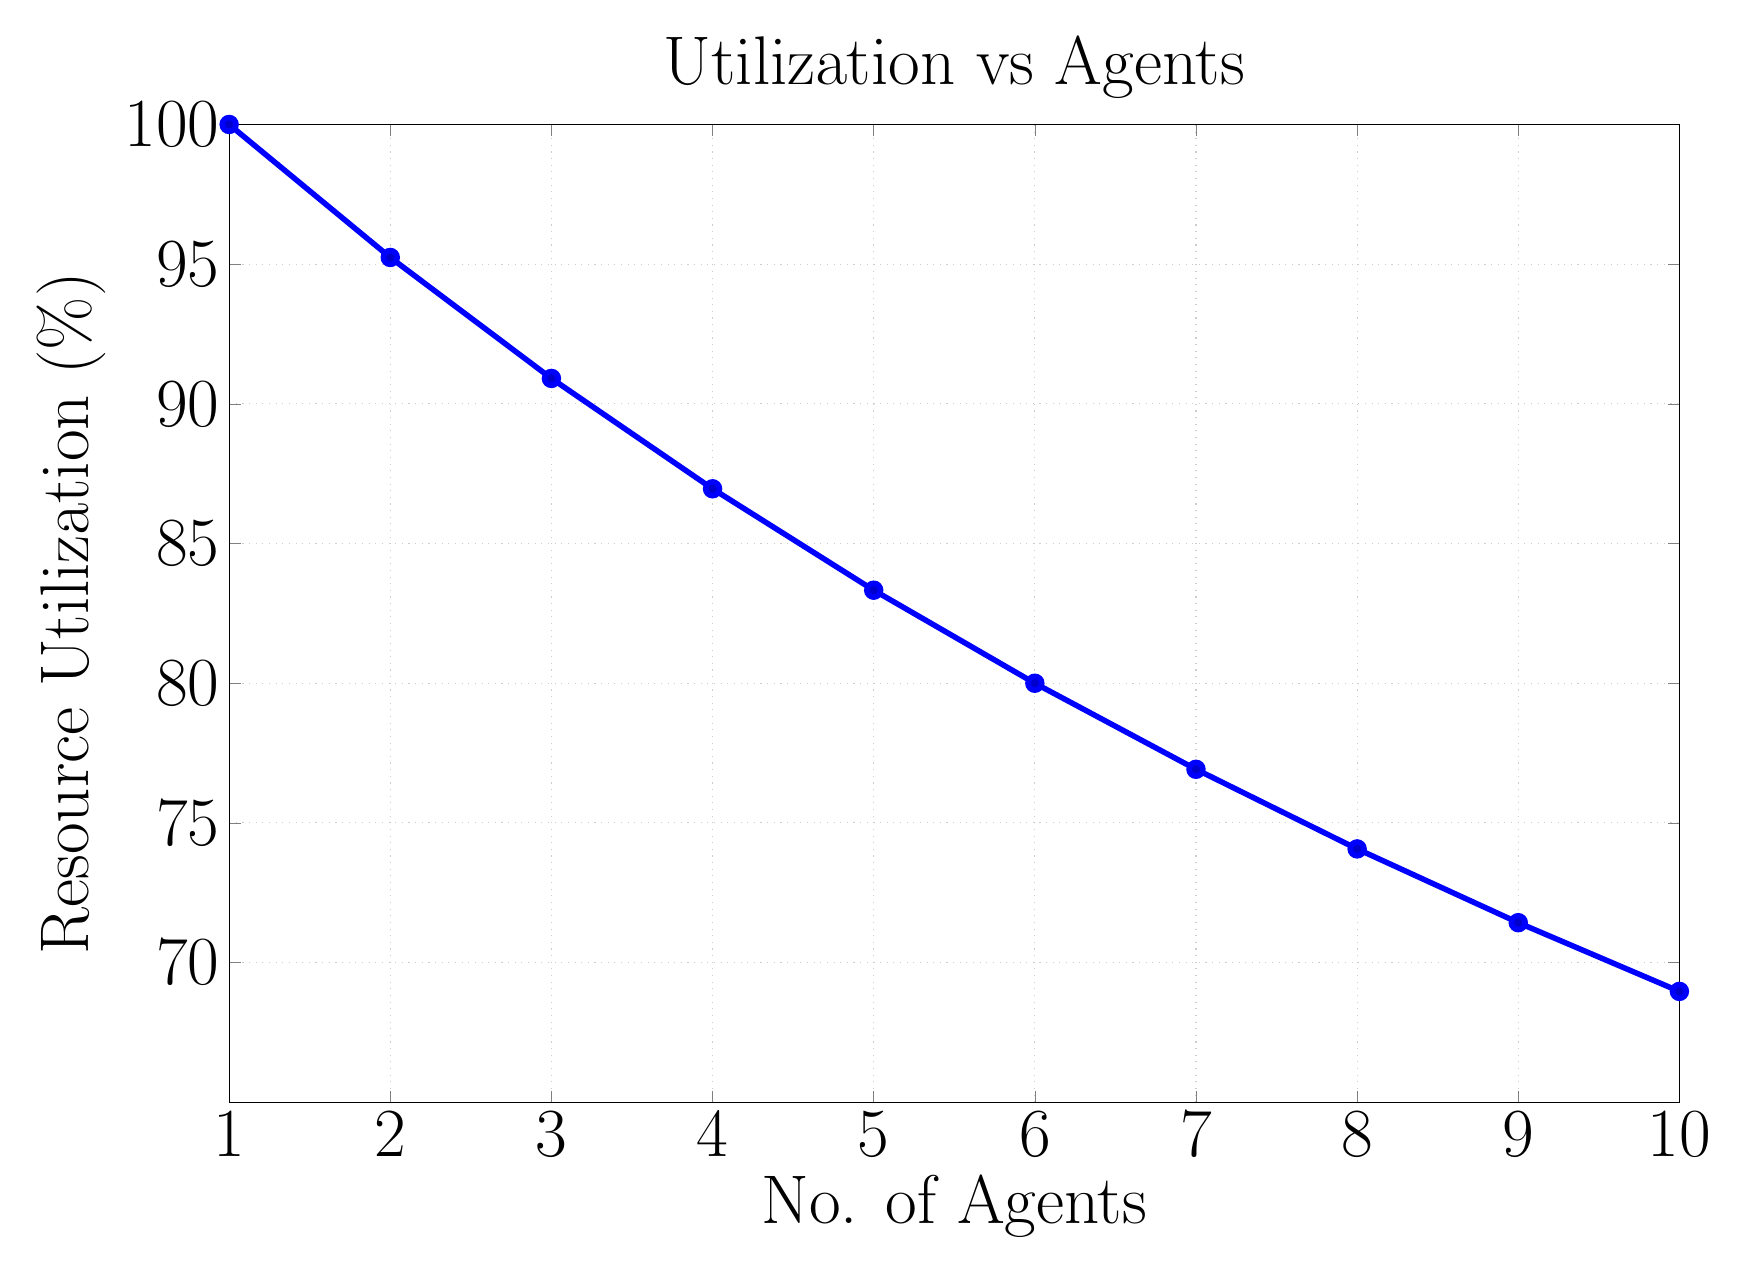
\begin{tikzpicture}
		\begin{axis}[
			width=20cm,
			height=14cm,
			tick label style={font=\fontsize{24}{28}\selectfont},
			label style={font=\fontsize{24}{28}\selectfont},
			title style={font=\fontsize{24}{28}\selectfont},
			xlabel={No. of Agents},
			ylabel={Resource Utilization (\%)},
			title={Utilization vs Agents},
			xmin=1, xmax=10,
			ymin=65, ymax=100,
			xtick={1,2,3,4,5,6,7,8,9,10},
			ytick={70,75,80,85,90,95,100},
			grid=both,
			grid style={dotted, gray!40},
		]
			
			\addplot+[mark=*, color=blue, line width=2pt, mark size=2.5pt] coordinates {
				(1,100.00)(2,95.24)(3,90.91)(4,86.96)(5,83.33)(6,80.00)(7,76.92)(8,74.07)(9,71.43)(10,68.97)
			};
			
		\end{axis}
	\end{tikzpicture}
\end{document}
